
\section{Supplementary Video}
\subsection{Supplementary Video S1.}
\label{video}
\href{https://youtu.be/Ee2sU-AZWC4}{\textbf{youtu.be/Ee2sU-AZWC4}}
provides a high-level overview of the results reported in this paper.





\section{Supplementary Discussion}
\label{sec:supplementary-discussion}



\subsection{Embodiment.}

We consider an agent to be embodied if its output affects its input.
This relationship may be represented by the simple update rule $\ell_{t+1} = f(\ell_t,\, \phi)$,
where $\ell_t$ denotes the morphology of an agent at time $t$, and $\phi$ denotes its control policy.
In a disembodied system, changes to the morphology are not directly constrained by its current state; the update rule becomes: $\ell_{t+1} = f(\phi)$.

Once a round robot begins rolling, its control policy cannot instantaneously force the system to go in the other direction, since
momentum will tend to preserve forward movement.
This has the effect of reducing selection pressure on the controller, since fewer variations are deleterious.
This allows evolution to continue climbing fitness gradients by mutating the controllers within these permissive body plans.

This might also be possible in disembodied agents if other dimensions of the system can be changed by some search process such as to facilitate the search for $\phi$.



\section{Supplementary Methods}
\label{sec:supplementary-methods}

\subsection{Rigid-bodied robots.}

Rigid-bodied robots and their environment were simulated using Pyrosim
(\href{https://ccappelle.github.io/pyrosim/}{ccappelle.github.io/pyrosim}).
% \cite{kriegman2017simulating}.
The robot is a quadruped with a large, spherical abdomen; each leg is attached by a single degree-of-freedom hinge joint.\\[0.75em]
\centerline{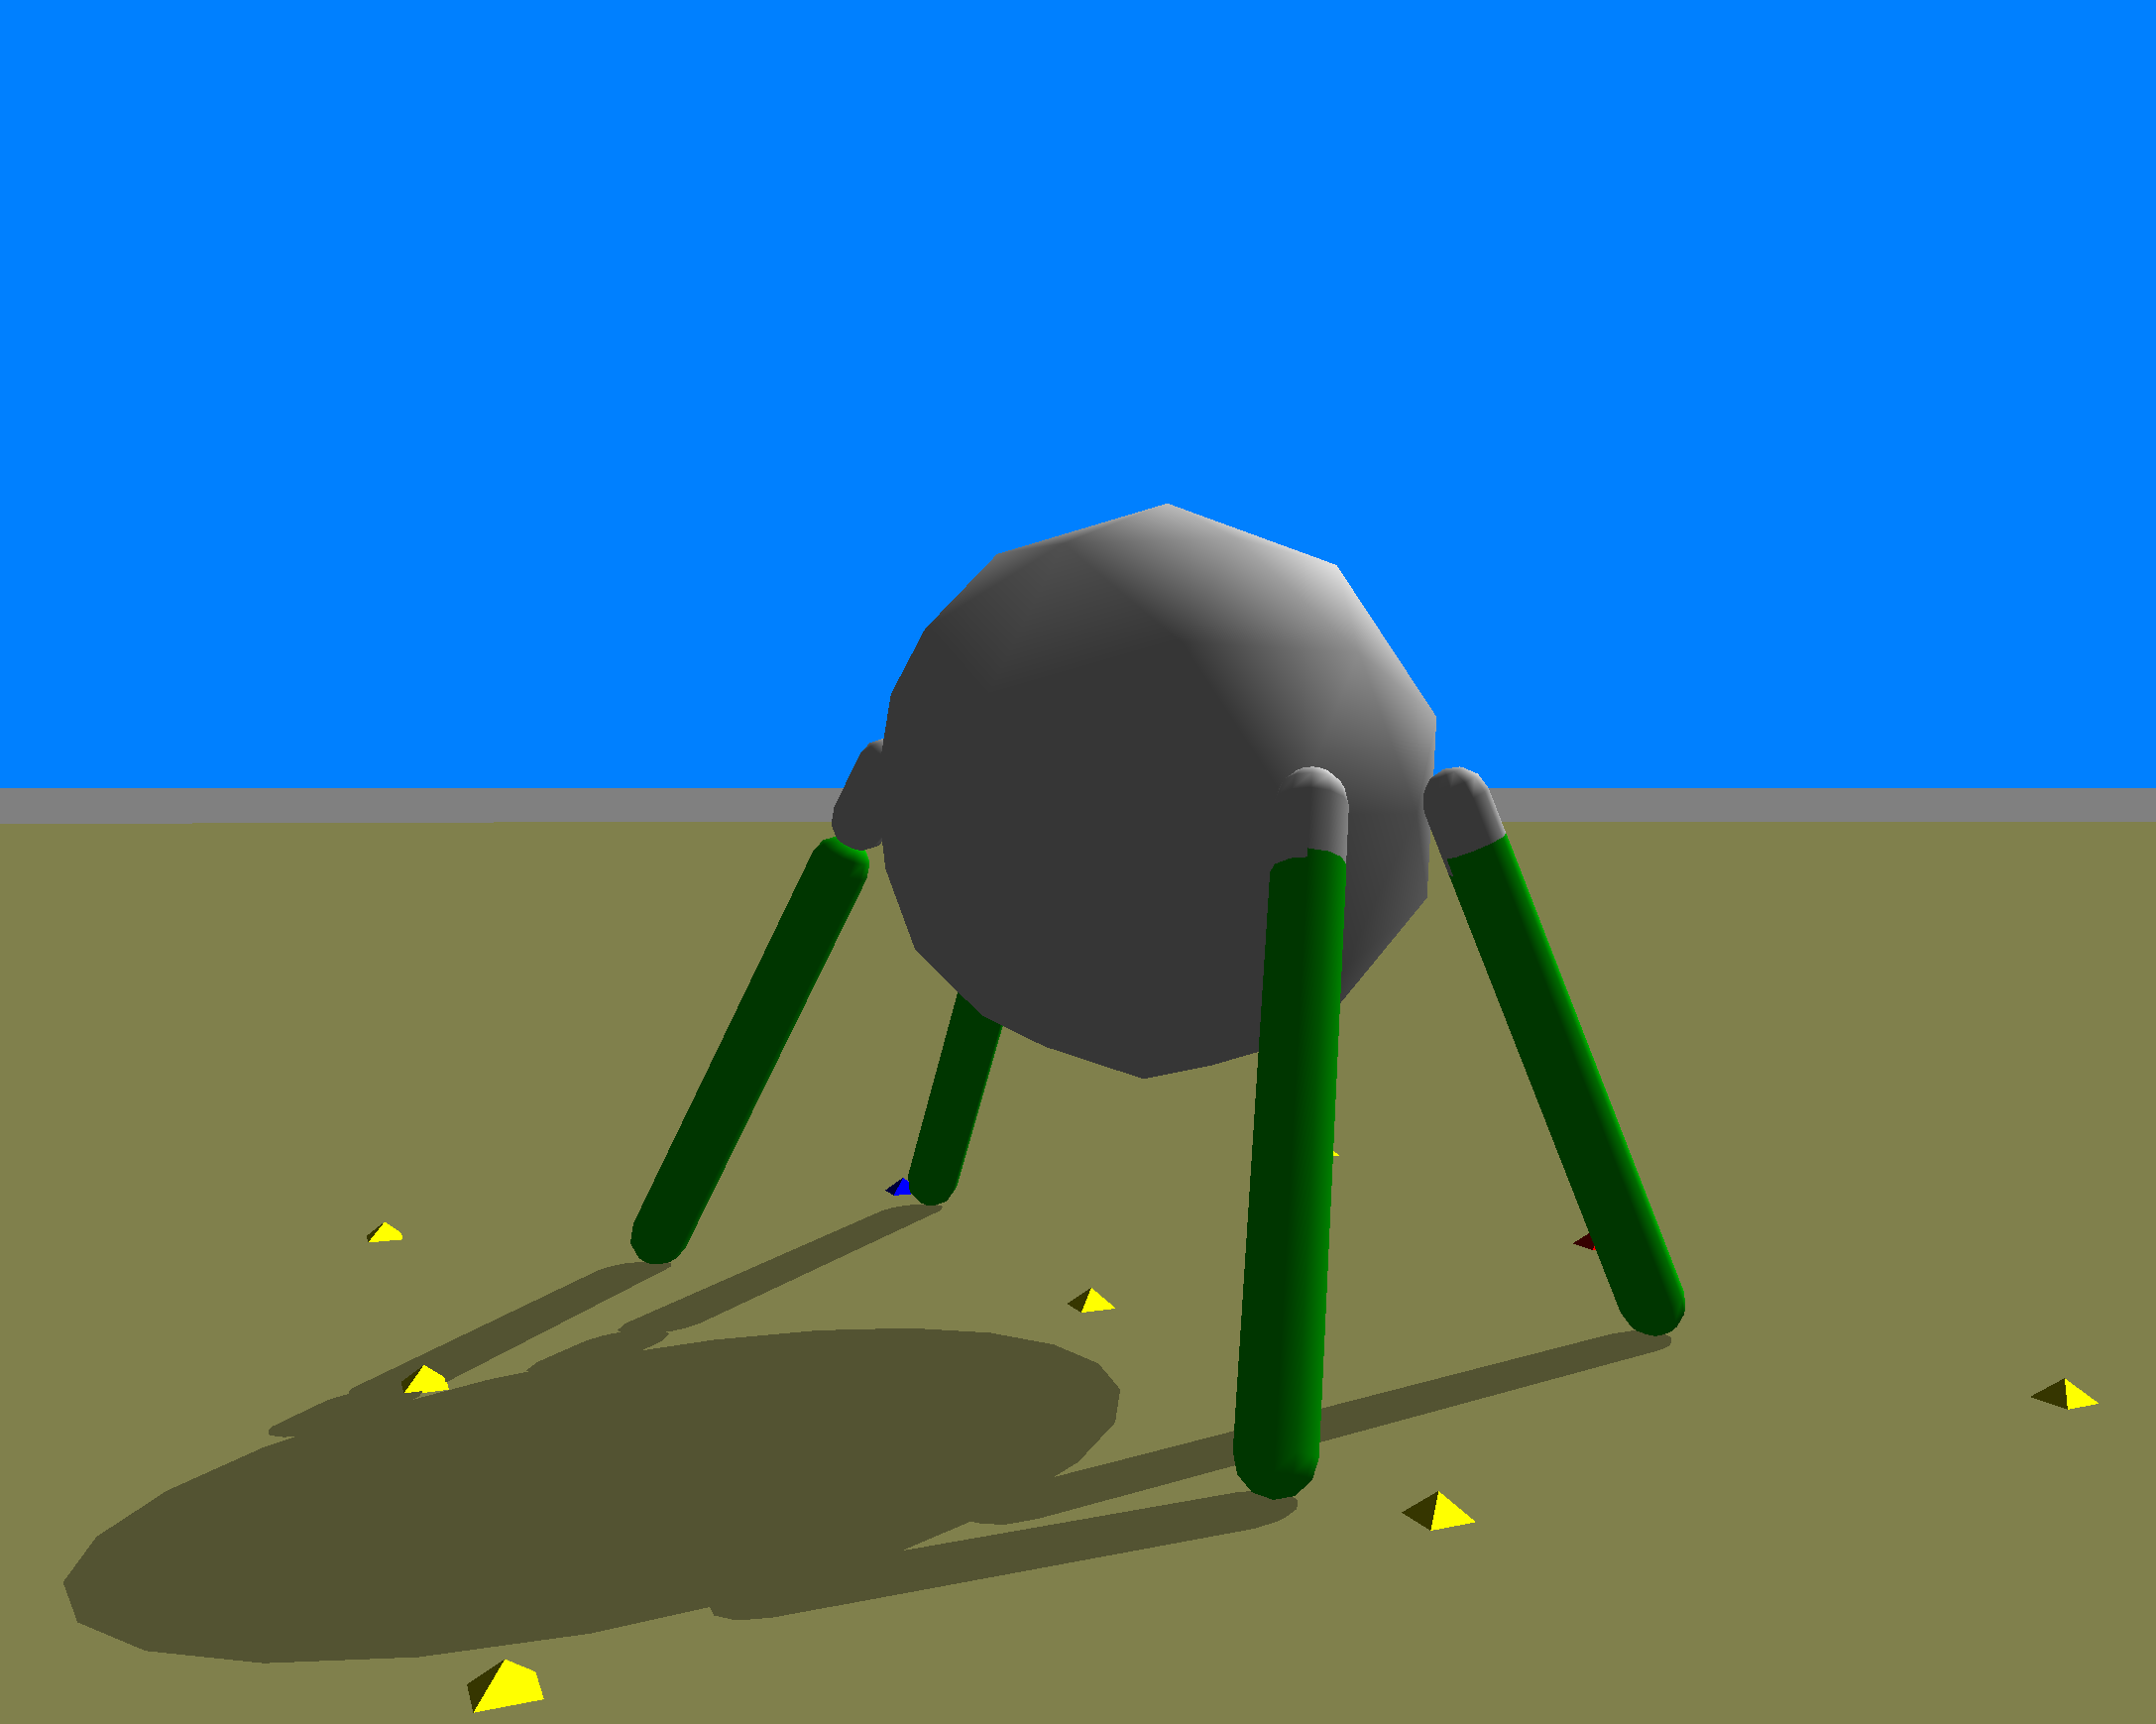
\includegraphics[width=0.4\linewidth]{Chapter04/rigid-body.png}}

\vspace{0.75em}
Morphological development was approximated in rigid bodies using linear actuators to slowly lengthen or shorten the length of each leg, from an evolved starting value (between 0 and 1) to an evolved final value (between 0 and 1).
The controller is a simple neural net: two central pattern generators are fully connected to four motor neurons, each of which innervate a separate hinge joint.
Controller development was approximated in neural networks through ballistic change to each synaptic weight: As the simulation proceeds, each weight develops linearly, from an evolved starting value (between -1 and +1) to an evolved final value (between -1 and +1).


The genotype spans two arrays: one for initial and final synaptic weights (controller), and another for initial and final leg lengths (morphology). 
Mutations affect, on average, a single element in each array.
Apart from the genotype and its mutations, the evolutionary algorithm is identical to that of the soft robots.
However, the task environment now consists of a sloped floor, declined toward a light source; and
performance is measured by the average light intensity recorded by a light sensor embedded in the center of the agent's abdomen, according to the inverse square law of light propagation, at each time step in its life. Occlusion of the light caused by interference of the robot's own body parts was not simulated.


The results are presented below in Supplementary Fig. \hyperref[fig:S5]{S5}.


\subsection{Mutations for soft robots.}

The following derivation shows that there is a negligible difference in the mutations produced by the Evo and Evo-Devo treatments, in terms of the number of voxels modified (Fig. \hyperref[fig:S4]{S4}). 

Each voxel cell of a soft robot has its own material properties that can be changed by the evolutionary algorithm.
Evo voxels have two material properties: (1) resting length and (2) phase offset.
Evo-Devo voxels have four material properties: (1) initial resting length, (2) final resting length, (3) initial phase offset, and (4) final phase offset.


Mutations are applied by first choosing which material properties to mutate, and then choosing, separately for each property, which voxels to modify.
For each of the $n$ material properties, we select it with independent probability $p=1/n$. 
If none are selected, we randomly choose one. This occurs with probability $\left(1-p\right)^n$.
Hence the number of selected material properties for mutation is a random variable $S$ which follows a truncated binomial distribution,
\begin{equation}
\text{Pr}(S = s \mid n) = 
	\begin{cases} 
        0 & \text{ for } \;  s = 0 \\[4pt]
        n p(1-p)^{n-1} + (1-p)^n & \text{ for } \;  s = 1 \\[8pt]
        \dbinom{n}{s} p^s (1-p)^{n-s} & \text{ for } \;  s > 1
	\end{cases}
\end{equation}
The expected number of selected material properties is then:
\begin{align}
\mathbb{E}(S) 
&=
np(1-p)^{n-1} + (1-p)^n + \sum_{s=2}^n s \binom{n}{s} p^s (1-p)^{n-s} \\
&= 
(1-p)^n + \sum_{s=1}^n s \binom{n}{s} p^s (1-p)^{n-s} \\
&= 
(1-p)^n + np \\
&= 
(1-p)^n+1 .
\end{align}


For a selected material property, 
each voxel is mutated independently with probability $\lambda$, a hyperparameter we call the \textbf{mutation rate}.
The expected \textit{number} of genotype elements mutated given $K$ total voxels is thus:
\begin{equation}
\delta_{\text{gene}} = \lambda K \cdot \mathbb{E}(S) .
\end{equation}
Dividing by the length of the genome, $nK$, we get the expected \textit{proportion} of genotype elements mutated:
\begin{equation}
\pi_{\text{gene}} = \lambda/n \cdot \mathbb{E}(S).
\end{equation}
Note that imposing bilateral symmetry does not change these expected values.

We have $K=48$ total voxels, and $n=\{2,4\}$ material properties for our two main experimental treatments \{Evo, Evo-Devo\}, respectively. The expected difference between a robot and its offspring, in terms of genotype elements, is summarized in the following table.
\vspace{-1em}
\begin{table}[!ht]
\centering
\begin{tabular}{rcc}
 & $n=2$ & $n=4$  \\ \cline{2-3} 
\multicolumn{1}{r|}{$\delta_{\text{gene}}$}     & \multicolumn{1}{c|}{$60\lambda$}    & \multicolumn{1}{c|}{$63.8175\lambda$} \\ \cline{2-3} 
\multicolumn{1}{r|}{$\pi_{\text{gene}}$} & \multicolumn{1}{c|}{$0.625\lambda$} & \multicolumn{1}{c|}{$0.3291\lambda$}  \\ \cline{2-3} 
\end{tabular}
\end{table}

\noindent
However, because multiple material properties can be mutated within a single voxel, the expected number of voxels mutated is lower than the expected number of genotype elements mutated. 
To calculate the average number of voxels mutated we need to consider a hierarchy of binomial distributions.


Given that $S$ material properties were selected for mutation,
the number of material properties mutated within a single voxel, $M$ follows a binomial distribution, 
% $M\sim\text{binom} (S, \lambda)$,
\begin{equation}
\text{Pr}(M=m \mid S, \lambda) 
= 
\dbinom{S}{m} \lambda^m (1-\lambda)^{S-m} .
\end{equation}
For brevity, let's denote the probability that at least one mutation occurs within the voxel as $\theta$,
\begin{equation}
\theta = \text{Pr}(M>0 \mid S,\lambda)
=
1-(1-\lambda)^S .
\end{equation}
Then the number of voxels mutated, $V$, across a total of $K$ voxels and $S$ selected material properties, also follows a binomial distribution:
% binom$(K, \theta)$. 
\begin{equation}
\text{Pr}(V=v \mid S, K, \lambda, n) 
= 
\dbinom{K}{v} \theta^v (1-\theta)^{K-v}.
\end{equation}
And the expected number of voxels mutated (out of $K$ total) is
\begin{align}
\delta_{\text{vox}}
&=
\mathbb{E}(V \mid K, \lambda, n) \\
&=
\mathbb{E}_S \, \mathbb{E}_{V}(V \mid S, K, \lambda, n) \\
&= 
\mathbb{E}_S (K\theta \mid S, K, \lambda, n) \\
&=
K \left\{
1-\mathbb{E}_S \left[(1-\lambda)^S \mid \lambda, n\right] \right\} \\
&=
K \left\{ 1 - \left[ (1-\lambda)(1-p)^n
+  \sum_{s=1}^{n} (1-\lambda)^s \dbinom{n}{s} p^s (1-p)^{n-s}
 \right] \right\} \\
&=
K \left\{ 
1 - (1-p)^n \left[ \left(\frac{\lambda p-1}{p - 1}\right)^n - \lambda\right]
\right\} 
\end{align}

 
There is an extremely tight bound on the proportion of voxels mutated, $\pi_{\text{vox}} = \delta_{\text{vox}}/K$, for any $n > 1$  (Fig. \hyperref[fig:S4]{S4}).
Thus mutations in Evo $(n=2)$ and Evo-Devo $(n=4)$ have practically the same impact in terms of the number of voxels modified.
For completeness, the following table displays $\delta_{\text{vox}}$ for the specific values of $\lambda$ considered by our hyperparameter sweep ($K=48$) (Fig. \hyperref[fig:S3]{S3}). 
\vspace{-0.5em}
\begin{table}[h!]
\centering
\begin{tabular}{cccccccccc}
  & & \multicolumn{8}{c}{$\lambda$} \\ \cline{3-10}
  & \multicolumn{1}{c|}{}  & 1/48    & 2/48    & 4/48    & 8/48    & 16/48   & 24/48   & 32/48   & \multicolumn{1}{c|}{48/48} \\ \cline{2-10} 
\multicolumn{1}{c|}{\multirow{2}{*}{$n$}} & \multicolumn{1}{c|}{2} &
1.25 & 2.48 & 4.92 & 9.67 & 18.67 & 27 & 34.67 & \multicolumn{1}{c|}{48}    \\
\multicolumn{1}{c|}{}                     & \multicolumn{1}{c|}{4} & 
1.3 & 2.6 & 5.14 & 10.05 & 19.17 & 27.46 & 34.98 & \multicolumn{1}{c|}{48}    \\ \cline{2-10} 
\end{tabular}
\end{table}





